\section{Agent-Coordinated Task-Level Operation}
\label{sec:closed-loop-operation}

A task supplies a process objective and the active line, product, and run context. Fig.~\ref{fig:agent-loop} shows the conceptual task-to-write workflow; it does not depict a successful live-Agent run. Context alone does not authorize a device write. The control node is selected from an explicit \texttt{control\_node\_id} or the Agent's configured control-write or recipe binding. The data-acquisition (DAQ) target is selected from an explicit ID or Agent DAQ binding; a read-only node visible through the channel line is also eligible. Section~\ref{sec:eval} reports scripted process results separately from exploratory live-Agent episodes.

In goal mode, a Lead Agent may decompose the objective, dispatch worker subtasks, and assess completion; this optional coordination does not define a control policy. For each step, the responsible Agent invokes \texttt{optimization\_explore}, which checks the request before device I/O.

The operation resolves the optimization profile and control-node binding, then uses the node's stored value as the current setpoint $u_0$. This value is not necessarily a fresh device readback. If direction is omitted, the operation defaults to an upward adjustment; otherwise, the supplied direction sets $s\in\{-1,+1\}$. For a step $\Delta u$, it forms
\begin{equation}
 u^{*}=\operatorname{clip}\!\left(u_0+s\Delta u,\,u_{\min},\,u_{\max}\right),
 \label{eq:optimization-candidate}
\end{equation}
where configured tuning bounds take precedence; node bounds are used otherwise. The effective step is selected in this order: an explicit argument, the binding's tuning step, the scene's maximum step, or one twentieth of the node range.

The operation also resolves the DAQ target and checks its visibility. A subsequent implementation adds two configurable preflights. The identifiability check blocks a new step when the control node's intervention ledger contains an unclosed prior intervention or an unexpired recommended window after an underpowered or confounded verdict. The model--ontology cross-check treats missing evidence as unknown and rejects confirmed conflicts on automatic requests; on the manual path, it does not itself block dispatch. If the checks pass, the operation attempts a pre-write DAQ read, whose mean may be unavailable. These later checks are not attributed to the earlier experiments, whose active services were not captured as a hermetic snapshot.

A valid candidate enters the shared write path, which resolves binding and authority and checks whether the route requires approval. Only gated routes wait; after approval, authorization and binding are revalidated. Before driver I/O, the common controller applies range limits and, for agent or manual writes outside benchmark mode, applicable step, timing, and hold constraints. Ungated routes skip approval but still pass these checks. A pre-dispatch denial is recorded as rejected without a driver call. A driver-stage error may occur after dispatch begins, so status alone cannot establish whether the device changed; state must be read and reconciled before retrying.

After a successful write, the operation waits for the configured settling interval (10--300~s; 45~s by default) and attempts a post-write DAQ read. A subsequent implementation defines the pre- and post-write windows as $[t_0-\tau,t_0]$ and $[t_0,t_1]$, where $t_0$ precedes the pre-write read/write call and $\tau$ is the settling interval. Because approval can delay dispatch, the latter window may include pre-dispatch samples; its mean alone is not causal. The earlier implementation instead reads trailing 45-s windows. Neither definition establishes causation.

The exploration record retains the control value (the target after a successful write), step, available DAQ means, and write status/message. A rejected attempt has no separate attempted-target field. The shared path records the command outcome and any device readback separately. On a later task turn, the Agent can review the result, choose another direction and step, or stop. The runtime therefore depends on a subsequent Agent decision; it does not iterate autonomously to convergence. Fig.~\ref{fig:agent-loop} summarizes these branches and separates command records from later process feedback.

\begin{figure*}[!t]
\centering
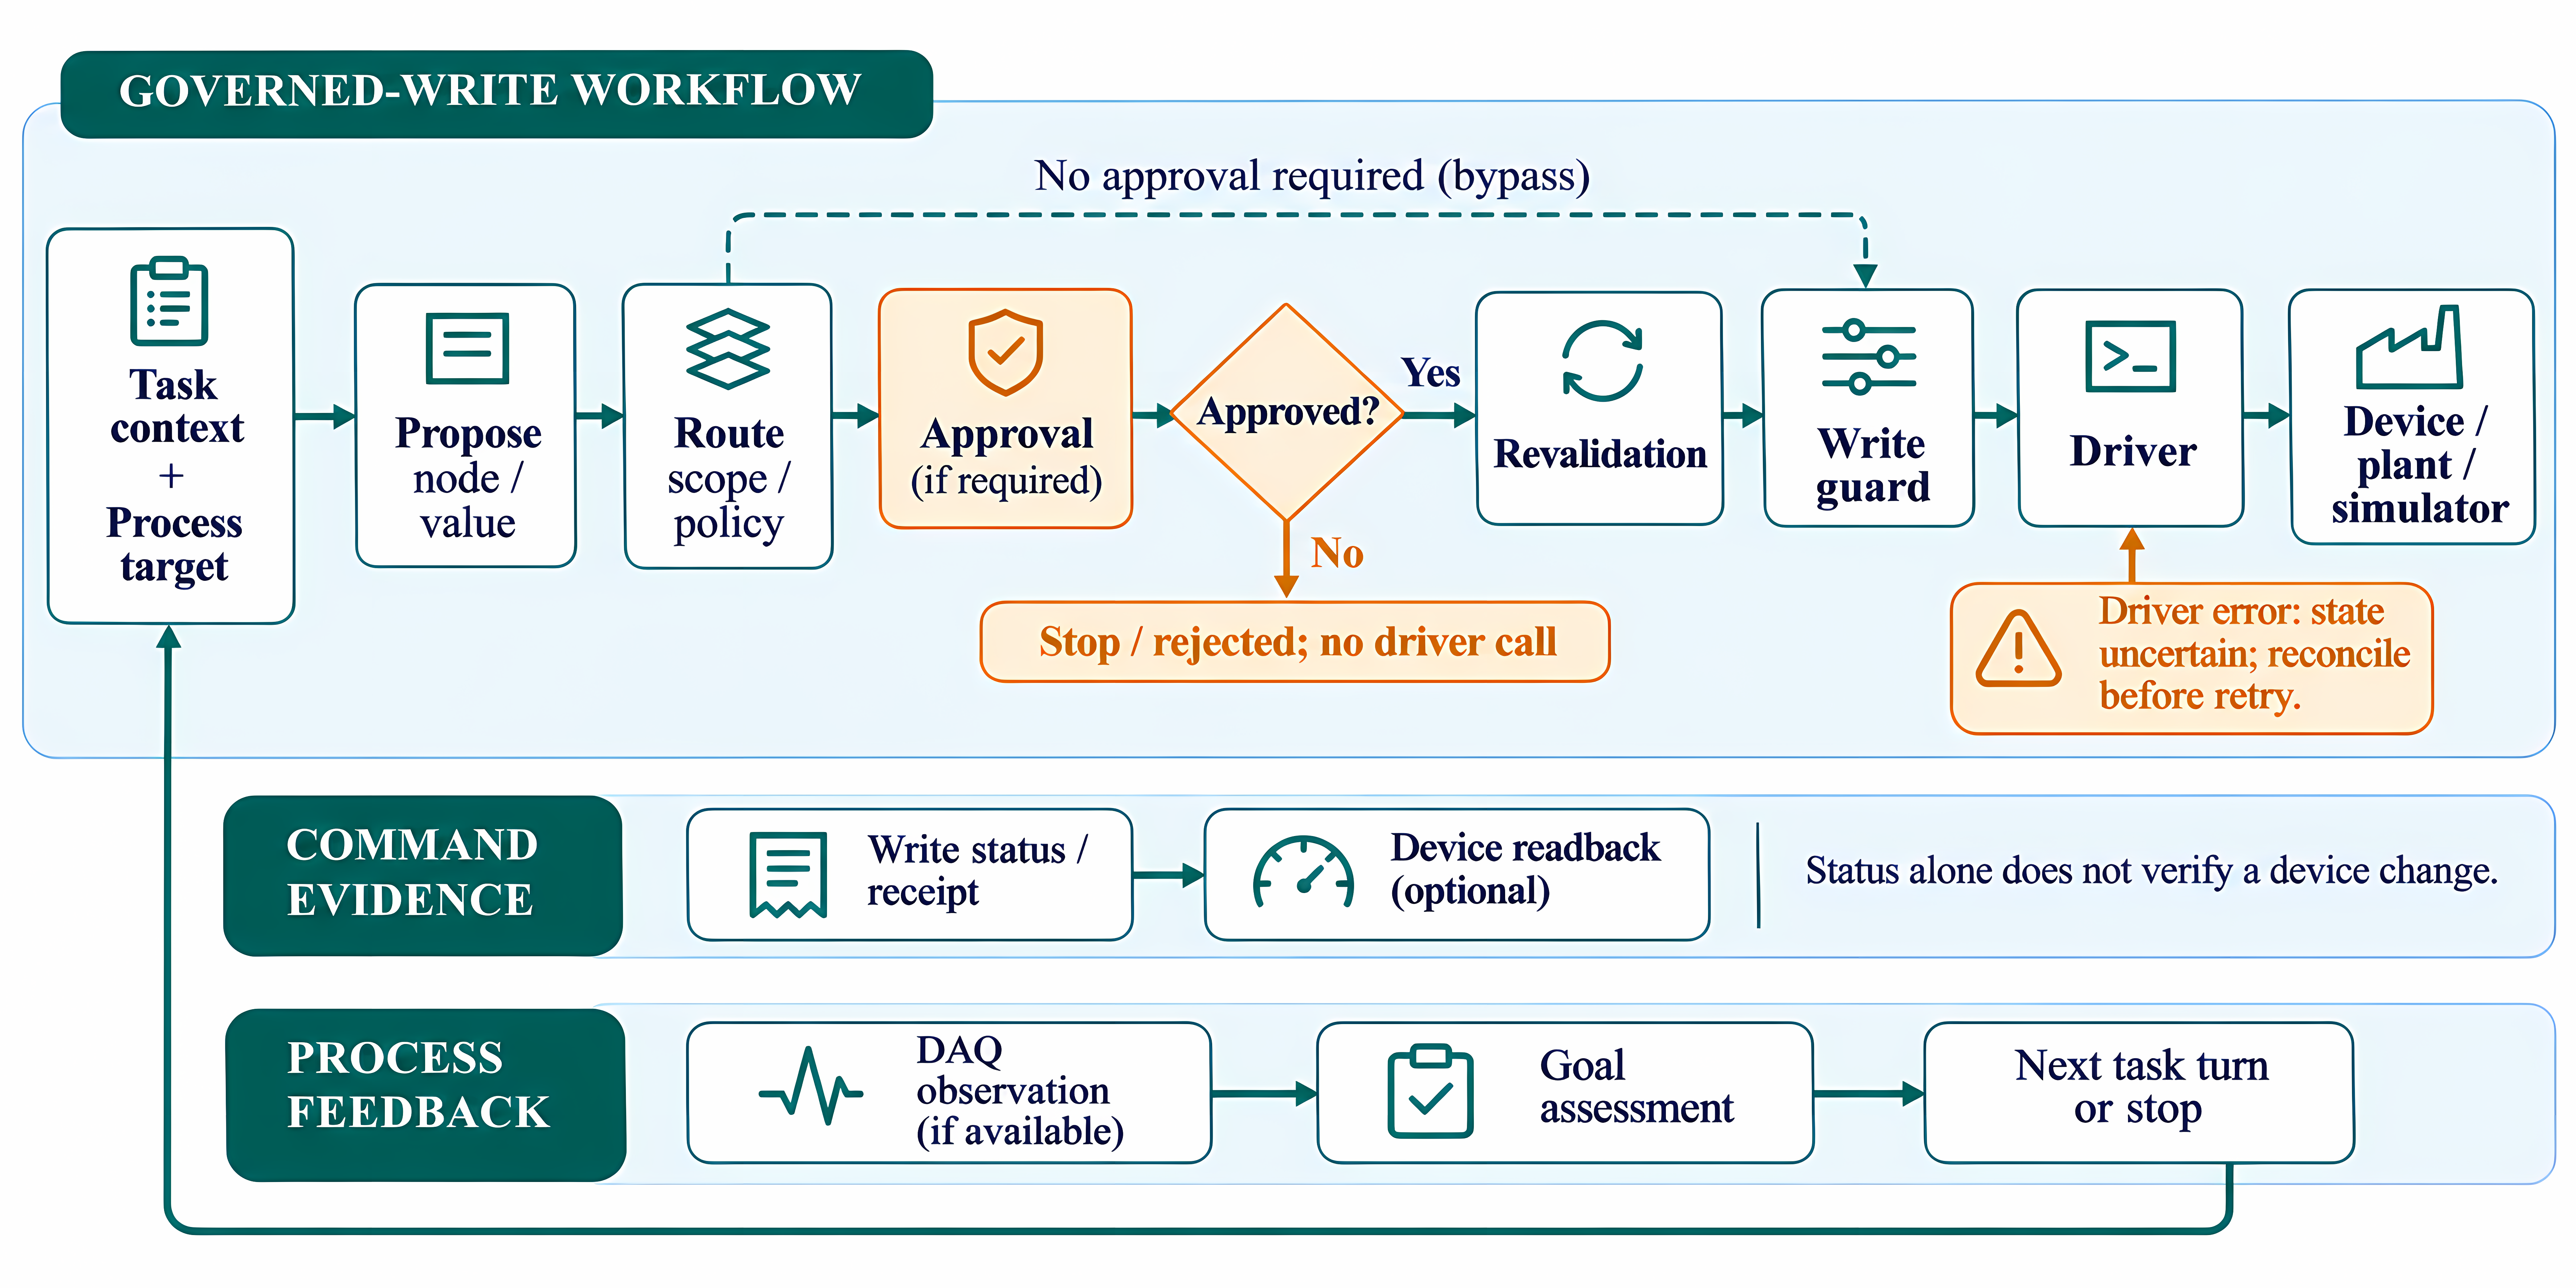
\includegraphics[width=\textwidth]{../figures/fig3.png}
\caption{Conceptual governed-write workflow. The task context supplies a process goal, and the Agent proposes a node/value that passes route-scope and policy checks. Requests requiring approval proceed through the decision and, if approved, revalidation; requests that do not require approval bypass those stages but still enter the write guard. Rejection stops before any driver call. A driver-stage error may leave device state uncertain and require reconciliation. The figure separates a write status/receipt and optional device readback from later DAQ feedback and goal assessment on a subsequent task turn. It describes the workflow, not an observed live-Agent success.}
\label{fig:agent-loop}
\end{figure*}
